% This file: 			Draft Compiling New Information and Analysis
% Contributors: 		Pietro Biroli, Daniela Del Boca, Linor Kiknadze, 
%					Yu Kyung Koh, Sylvi Kuperman, Sidharth Moktan, 
%					Chiara Pronzato, Anna Ziff
% Original date: 		10/3/16
% Project: 			Reggio Evaluation

\documentclass[12pt]{article}
\usepackage[top=1in, bottom=1in, left=1in, right=1in]{geometry}
\parindent 22pt

\usepackage{adjustbox}
\usepackage{amsmath}
\usepackage{amssymb}
\usepackage{array}
\usepackage{booktabs}
\usepackage{datetime}
\usepackage{fancyhdr}
\usepackage{float}
\usepackage{graphicx}
\usepackage[colorlinks=true,linkcolor=blue,urlcolor=blue,anchorcolor=blue,citecolor=blue]{hyperref}
\usepackage{lscape}
\usepackage{multirow}
\usepackage{natbib}
\usepackage{setspace}
\usepackage{tabularx}
\usepackage[colorinlistoftodos,linecolor=black]{todonotes}
\usepackage{appendix}
\usepackage{pgffor}
\usepackage{caption} 
\usepackage{threeparttable}
\captionsetup[table]{skip=3pt}

\settimeformat{hhmmsstime}

\newcolumntype{L}[1]{>{\raggedright\arraybackslash}p{#1}}
\newcolumntype{C}[1]{>{\centering\arraybackslash}p{#1}}
\newcolumntype{R}[1]{>{\raggedleft\arraybackslash}p{#1}}

\begin{document}
\doublespacing

\section{Sensitivity Analysis}

While checking data, we have come across several interviewers that show some trends in questionable recordings on school assignment. Table \ref{tab:num-interview} reports the number of interviews each interviewer did. Table \ref{tab:question-interviewers} reports ID's of the questionable interviewers and examples of concerns noted for each interviewers. 

Since dropping all the questionable interviewers significantly decreases sample size so that the statistical power is lost, we carry out alternative sensitivity analysis as follows. We select two outcomes for each age cohort, and run OLS regression with treatment indicator and BIC-selected control set dropping each of all interviewers. Sample is limited to people in Reggio Emilia only. We explore how the coefficient on treatment indicator changes when we drop different interviewers. Figures \ref{fig:child-sensitivity-interviewer} - \ref{fig:adult40-sensitivity-interviewer} plot the OLS coefficient on the treatment indicator and its standard error for each case of dropping interviewer marked on the horizontal axis.

\begin{table}[H] \caption{Number of Interviews by Each Interviewer} \label{tab:num-interview}
\scalebox{0.8}{\begin{tabular}{*{5}{c} C{.5cm} *{5}{c}} \\
\cline{1-5} \cline{7-11} \\[-5pt]
 Interviewer & Reggio & Parma & Padova & Total && Interviewer & Reggio & Parma & Padova & Total \\
\cline{1-5} \cline{7-11}
 166 & . & . & 4 & 4 && 4014 & . & 13 & . & 13 \\[3pt] 
 167 & 20 & 54 & . & 74 && 4015 & . & 5 & . & 5 \\[3pt] 
 168 & . & 7 & . & 7 && 4017 & . & 4 & . & 4 \\[3pt] 
 169 & . & 1 & . & 1 && 4018 & 126 & 264 & . & 390 \\[3pt] 
 170 & 111 & 3 & . & 114 && 4019 & . & 12 & . & 12 \\[3pt] 
 171 & 122 & . & 8 & 130 && 4020 & . & 3 & . & 3 \\[3pt] 
 172 & 91 & . & . & 91 && 4026 & . & 8 & . & 8 \\[3pt] 
 173 & 119 & . & . & 119 && 4035 & . & . & 56 & 56 \\[3pt] 
 176 & . & . & 35 & 35 && 4037 & . & . & 118 & 118 \\[3pt] 
 177 & . & . & 47 & 47 && 4040 & . & . & 24 & 24 \\[3pt] 
 178 & . & . & 11 & 11 && 4041 & . & . & 8 & 8 \\[3pt] 
 183 & . & 10 & . & 10 && 4042 & . & . & 26 & 26 \\[3pt] 
 184 & 87 & 99 & 46 & 232 && 4043 & . & . & 70 & 70 \\[3pt] 
 185 & 64 & 15 & 81 & 160 && 4044 & . & . & 41 & 41 \\[3pt] 
 186 & 39 & 113 & 23 & 175 && 4045 & . & . & 21 & 21 \\[3pt] 
 187 & 49 & 47 & 29 & 125 && 4046 & . & . & 34 & 34 \\[3pt] 
 192 & . & . & 16 & 16 && 4047 & . & . & 6 & 6 \\[3pt] 
 193 & . & . & 36 & 36 && 4053 & 4 & . & . & 4 \\[3pt] 
 195 & . & . & 7 & 7 && 4054 & 39 & . & . & 39 \\[3pt] 
 196 & . & . & 5 & 5 && 4056 & 19 & . & . & 19 \\[3pt] 
 855 & 8 & . & . & 8 && 4057 & 6 & . & . & 6 \\[3pt] 
 1369 & . & . & 20 & 20 && 4058 & 13 & . & . & 13 \\[3pt] 
 2437 & . & 1 & 86 & 87 && 4059 & 35 & . & . & 35 \\[3pt] 
 2502 & . & . & 7 & 7 && 4060 & 25 & . & . & 25 \\[3pt] 
 2506 & . & . & 28 & 28 && 4063 & 21 & . & . & 21 \\[3pt] 
 2509 & . & . & 22 & 22 && 4065 & 80 & . & . & 80 \\[3pt] 
 2511 & . & . & 30 & 30 && 4072 & . & 8 & . & 8 \\[3pt] 
 2525 & . & . & 35 & 35 && 4073 & . & 217 & . & 217 \\[3pt] 
 2526 & 59 & . & 81 & 140 && 4075 & . & 6 & . & 6 \\[3pt] 
 2544 & . & . & 144 & 144 && 4076 & 7 & . & . & 7 \\[3pt] 
 2562 & 20 & . & . & 20 && 4077 & 92 & . & . & 92 \\[3pt] 
 2593 & . & . & 21 & 21 && 4078 & 16 & . & . & 16 \\[3pt] 
 2594 & . & . & 18 & 18 && 4082 & 27 & . & . & 27 \\[3pt] 
 2596 & . & . & 16 & 16 && 4087 & . & 10 & . & 10 \\[3pt] 
 2597 & . & . & 62 & 62 && 4089 & . & 10 & . & 10 \\[3pt] 
 2712 & . & 4 & . & 4 && 4091 & . & 226 & . & 226 \\[3pt] 
 2718 & 8 & . & . & 8 && 4092 & . & 4 & . & 4 \\[3pt] 
 2747 & 65 & . & . & 65 && 4096 & . & 51 & . & 51 \\[3pt] 
 2752 & . & 7 & . & 7 && 4097 & . & 9 & . & 9 \\[3pt] 
 2753 & 114 & . & . & 114 && . & . & . & . & . \\[3pt] 
\hline
\end{tabular}
}
\end{table}

\begin{table}[H]
\begin{footnotesize}
\caption{Questionable Interviewers}\label{tab:question-interviewers}
\begin{tabular}{L{2cm} L{2cm} L{11cm}} 
\toprule						
Interviewer ID	&	Total \# of Interviews Conducted	&	Examples of Concerns Noted	\\	\midrule
170	&	114	&	There are cases where attendance at a school type is mentioned, school name is reported, and school address is reported for cohorts that could not have attended due to following reasons: a) that school was not yet constructed when they were eligible to attend; or b) the school they report existed on another street at the time they were eligible to attend. 	\\	\midrule
171	&	130	&	There are cases where attendance at a school type is mentioned, school name is reported, and school address is reported for cohorts that could not have attended due to following reasons: a) that school was not yet constructed when they were eligible to attend; or b) the school they report existed on another street at the time they were eligible to attend. 	\\	\midrule
172	&	92	&	There are cases where attendance at a school type is mentioned, school name is reported, and school address is reported for cohorts that could not have attended due to following reasons: a) that school was not yet constructed when they were eligible to attend; or b) the school they report existed on another street at the time they were eligible to attend. 	\\	\midrule
186	&	175	&	Reports that 23 people, all in the Age-30 Cohort, are living in Parma as adults but attended preschool in Reggio Emilia. The school type, school name, and school address are all reported. None of the 23 is unable to provide a name or address. Another concern noted for this interviewer includes 17 observations in which all report attending the same school name on the same address but none of the 17 can report the actual school name (just "Comunale Stirone" referencing the school type and street address Stirone)	\\	\midrule
4018	&	390	&	This interviewer worked a lot in Parma, and we do not have municipal archives for school enrollment, thus we cannot be 100\% certain that the observations are questionable. because we cannot reconstruct the history of each school (i.e. date opened, school type, school address, whether rebuilt under a new name, etc). Some concerns are observations that conflict with the history provided by Parma, for example, reporting attendance at an asilo before asilos were first created. Another concern  is the total number of people who report a school name and address for a school that didn't yet exist or existed under a different name when the respondent was eligible to attend. The pattern of these errors is questionable.  In Reggio, there are fewer concerns with this interviewer.	\\	\midrule
4073	&	217	&	This interviewer worked exclusively in Parma, for which we have no municipal archives. One concern is the very unusual number of observations in which no school name is reported, but an address is provided; for Adolescents and Age-30 cohorts, this is very surprising. For Age 40 and 50, it is less surprising, but still this pattern is very different from the observations of other interviewers. Regardless, without a complete history of Parma, it's not possible to assign school types by street address or neighborhood alone as several different types of schools are generally in the same neighborhood or street.	\\	\bottomrule

\end{tabular}

\end{footnotesize}
\end{table}


\subsection{Within Reggio Emilia Analysis} \label{sec:within-RE-analysis}

    \begin{figure}[H]
      \centering
        \begin{subfigure}[t]{0.75\textwidth}
          \includegraphics[width=\textwidth]{../../../output/image/coef-interviewer-child-pos_childSDQ_score.eps}       
\caption{Outcome: Positive SDQ Score}        
        \end{subfigure}
        \begin{subfigure}[t]{0.75\textwidth}
          \includegraphics[width=\textwidth]{../../../output/image/coef-interviewer-child-BMI_obese.eps}       
 \caption{Outcome: Not Obese}        
        \end{subfigure}
      \caption{Child Cohort: Droping Each Interviewer, Within Reggio Emilia Analysis}  \label{fig:child-sensitivity-interviewer}
    \end{figure}

    \begin{figure}[H]
      \centering
        \begin{subfigure}[t]{0.75\textwidth}
          \includegraphics[width=\textwidth]{../../../output/image/coef-interviewer-adol-pos_childSDQ_score.eps}       
\caption{Outcome: Positive SDQ Score}        
        \end{subfigure}
        \begin{subfigure}[t]{0.75\textwidth}
          \includegraphics[width=\textwidth]{../../../output/image/coef-interviewer-adol-BMI_obese.eps}       
 \caption{Outcome: Not Obese}        
        \end{subfigure}
      \caption{Adolescent Cohort: Droping Each Interviewer, Within Reggio Emilia Analysis}  \label{fig:adol-sensitivity-interviewer}
    \end{figure}


    \begin{figure}[H]
      \centering
        \begin{subfigure}[t]{0.75\textwidth}
          \includegraphics[width=\textwidth]{../../../output/image/coef-interviewer-adult30-votoMaturita.eps}       
\caption{Outcome: High School Grade}        
        \end{subfigure}
        \begin{subfigure}[t]{0.75\textwidth}
          \includegraphics[width=\textwidth]{../../../output/image/coef-interviewer-adult30-BMI_obese.eps}       
 \caption{Outcome: Not Obese}        
        \end{subfigure}
      \caption{Adult-30 Cohort: Droping Each Interviewer, Within Reggio Emilia Analysis}  \label{fig:adult30-sensitivity-interviewer}
    \end{figure}


    \begin{figure}[H]
      \centering
        \begin{subfigure}[t]{0.75\textwidth}
          \includegraphics[width=\textwidth]{../../../output/image/coef-interviewer-adult40-votoMaturita.eps}       
\caption{Outcome: High School Grade}        
        \end{subfigure}
        \begin{subfigure}[t]{0.75\textwidth}
          \includegraphics[width=\textwidth]{../../../output/image/coef-interviewer-adult40-BMI_obese.eps}       
 \caption{Outcome: Not Obese}        
        \end{subfigure}
      \caption{Adult-40 Cohort: Droping Each Interviewer, Within Reggio Emilia Analysis}  \label{fig:adult40-sensitivity-interviewer}
    \end{figure}


\subsubsection{More Detailed Analysis}

\ref{sec:within-RE-analysis} shows some interviewers that show different trend than other interviewers. For child and adolescent cohort, interviewers 2526 and 4018 show different results for outcomes examined. In order to examine this more closely, we estimate treatment effects excluding those interviewers on all main outcomes presented in the paper. 

\begin{table}[H] \caption{Estimation Results for Main Outcomes, Child Cohort} \label{ols-M-child-sensitivity}
\scalebox{0.7}{\begin{tabular}{l c c c c}
\toprule
 & None & Drop2526 & Drop4018 & DropAll \\
\midrule
IQ Factor & \textbf{ -0.19 } & -0.05 & \textbf{ -0.25 } & -0.11 \\
& (0.10) & (0.10) & (0.12) & (0.12) \\
& \textit{ 308 } & \textit{ 266 } & \textit{ 256 } & \textit{ 214 } \\
SDQ Composite - Child & \textbf{ 1.50 } & \textbf{ 1.05 } & \textbf{ 1.88 } & \textbf{ 1.42 } \\
& (0.54) & (0.58) & (0.59) & (0.65) \\
& \textit{ 307 } & \textit{ 265 } & \textit{ 255 } & \textit{ 213 } \\
Not Obese & -0.07 & 0.02 & -0.07 & 0.04 \\
& (0.05) & (0.05) & (0.06) & (0.06) \\
& \textit{ 308 } & \textit{ 266 } & \textit{ 256 } & \textit{ 214 } \\
Not Overweight & -0.01 & -0.01 & -0.01 & -0.03 \\
& (0.04) & (0.05) & (0.05) & (0.06) \\
& \textit{ 308 } & \textit{ 266 } & \textit{ 256 } & \textit{ 214 } \\
Health is Good & -0.01 & -0.04 & -0.02 & -0.06 \\
& (0.05) & (0.06) & (0.06) & (0.07) \\
& \textit{ 307 } & \textit{ 265 } & \textit{ 255 } & \textit{ 213 } \\
Not Excited to Learn & -0.01 & -0.00 & -0.00 & 0.01 \\
& (0.02) & (0.02) & (0.02) & (0.03) \\
& \textit{ 308 } & \textit{ 266 } & \textit{ 256 } & \textit{ 214 } \\
Problems Sitting Still & 0.01 & 0.03 & 0.02 & 0.05 \\
& (0.04) & (0.04) & (0.05) & (0.05) \\
& \textit{ 308 } & \textit{ 266 } & \textit{ 256 } & \textit{ 214 } \\
How Much Child Likes School & \textbf{ 0.11 } & 0.08 & \textbf{ 0.15 } & 0.11 \\
& (0.07) & (0.07) & (0.08) & (0.09) \\
& \textit{ 306 } & \textit{ 264 } & \textit{ 254 } & \textit{ 212 } \\
Num. of Friends & \textbf{ -0.41 } & \textbf{ -0.42 } & \textbf{ -0.47 } & \textbf{ -0.47 } \\
& (0.25) & (0.28) & (0.27) & (0.31) \\
& \textit{ 302 } & \textit{ 261 } & \textit{ 253 } & \textit{ 212 } \\
Candy Game: Willing to Share Candies & 0.00 & -0.02 & 0.04 & 0.03 \\
& (0.04) & (0.04) & (0.04) & (0.04) \\
& \textit{ 308 } & \textit{ 266 } & \textit{ 256 } & \textit{ 214 } \\
\bottomrule
\end{tabular}
}
\vspace{1ex} \\
\footnotesize\raggedright{\underline{Note 1:} This table shows the estimates of the coefficient for attending Reggio Approach preschools, checking for sensitivity regarding questionable interviewers. Column names indicate the interviewers being dropped. ``DropAll" columns drop all interviewers identified as questionable interviewers in the previous columns.}

\footnotesize\raggedright{\underline{Note 2:} Both unadjusted p-value and stepdown p-value are reported. Bold indicates that the estimate is significant at 10\% level.}
\end{table}


\begin{table}[H] \caption{Estimation Results for Main Outcomes, Adolescent Cohort} \label{ols-M-adol-sensitivity}
\scalebox{0.7}{\begin{tabular}{l c c c c}
\toprule
 & None & Drop2526 & Drop4018 & DropAll \\
\midrule
IQ Factor & -0.10 & 0.08 & -0.10 & 0.09 \\
& (0.10) & (0.08) & (0.13) & (0.11) \\
& \textit{ 292 } & \textit{ 275 } & \textit{ 233 } & \textit{ 216 } \\
SDQ Composite - Child & 0.24 & 0.17 & 0.51 & 0.44 \\
& (0.66) & (0.68) & (0.81) & (0.84) \\
& \textit{ 292 } & \textit{ 275 } & \textit{ 233 } & \textit{ 216 } \\
SDQ Composite & \textbf{ 1.04 } & 0.90 & 1.09 & 1.01 \\
& (0.69) & (0.72) & (0.78) & (0.81) \\
& \textit{ 290 } & \textit{ 273 } & \textit{ 231 } & \textit{ 214 } \\
Depression Score - positive & \textbf{ 2.34 } & \textbf{ 1.98 } & \textbf{ 2.40 } & \textbf{ 2.07 } \\
& (0.85) & (0.88) & (0.93) & (0.96) \\
& \textit{ 285 } & \textit{ 268 } & \textit{ 226 } & \textit{ 209 } \\
Locus of Control - positive & 0.11 & 0.05 & 0.07 & 0.00 \\
& (0.09) & (0.09) & (0.10) & (0.11) \\
& \textit{ 289 } & \textit{ 272 } & \textit{ 230 } & \textit{ 213 } \\
Not Obese & \textbf{ -0.09 } & -0.04 & -0.07 & -0.00 \\
& (0.05) & (0.04) & (0.05) & (0.05) \\
& \textit{ 292 } & \textit{ 275 } & \textit{ 233 } & \textit{ 216 } \\
Not Overweight & -0.02 & -0.02 & -0.04 & -0.05 \\
& (0.03) & (0.03) & (0.03) & (0.04) \\
& \textit{ 292 } & \textit{ 275 } & \textit{ 233 } & \textit{ 216 } \\
Health is Good & 0.06 & 0.04 & 0.07 & 0.05 \\
& (0.06) & (0.06) & (0.07) & (0.07) \\
& \textit{ 291 } & \textit{ 274 } & \textit{ 232 } & \textit{ 215 } \\
Go To School & 0.00 & -0.01 & 0.00 & -0.01 \\
& (0.02) & (0.02) & (0.03) & (0.03) \\
& \textit{ 292 } & \textit{ 275 } & \textit{ 233 } & \textit{ 216 } \\
How Much Child Likes School & -0.09 & -0.12 & -0.08 & -0.11 \\
& (0.12) & (0.13) & (0.14) & (0.14) \\
& \textit{ 279 } & \textit{ 264 } & \textit{ 220 } & \textit{ 205 } \\
Days of Sport (Weekly) & \textbf{ -0.48 } & -0.33 & -0.39 & -0.23 \\
& (0.26) & (0.27) & (0.29) & (0.30) \\
& \textit{ 286 } & \textit{ 270 } & \textit{ 227 } & \textit{ 211 } \\
Num. of Friends & -0.40 & -0.09 & 0.88 & 1.11 \\
& (1.02) & (1.06) & (1.03) & (1.09) \\
& \textit{ 284 } & \textit{ 267 } & \textit{ 227 } & \textit{ 210 } \\
Volunteers & 0.01 & 0.04 & 0.02 & 0.04 \\
& (0.06) & (0.07) & (0.07) & (0.08) \\
& \textit{ 292 } & \textit{ 275 } & \textit{ 233 } & \textit{ 216 } \\
Trust Score & 0.02 & 0.14 & -0.11 & 0.03 \\
& (0.19) & (0.20) & (0.22) & (0.22) \\
& \textit{ 290 } & \textit{ 273 } & \textit{ 231 } & \textit{ 214 } \\
\bottomrule
\end{tabular}
}
\vspace{1ex} \\
\footnotesize\raggedright{\underline{Note 1:} This table shows the estimates of the coefficient for attending Reggio Approach preschools, checking for sensitivity regarding questionable interviewers. Column names indicate the interviewers being dropped. ``DropAll" columns drop all interviewers identified as questionable interviewers in the previous columns.}

\footnotesize\raggedright{\underline{Note 2:} Both unadjusted p-value and stepdown p-value are reported. Bold indicates that the estimate is significant at 10\% level.}
\end{table}




% =========================================== %
\subsection{Reggio-Parma DiD Analysis} \label{sec:ParmaDiD-analysis}

    \begin{figure}[H]
      \centering
        \begin{subfigure}[t]{0.75\textwidth}
          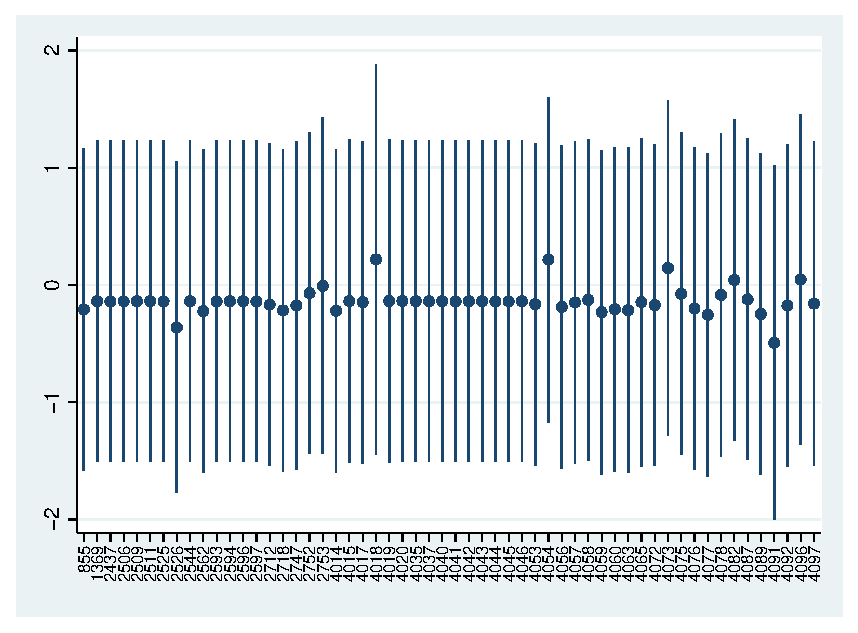
\includegraphics[width=\textwidth]{../../../output/image/coef-interviewer-child-pos_childSDQ_score_PmDiD.eps}       
\caption{Outcome: Positive SDQ Score}        
        \end{subfigure}
        \begin{subfigure}[t]{0.75\textwidth}
          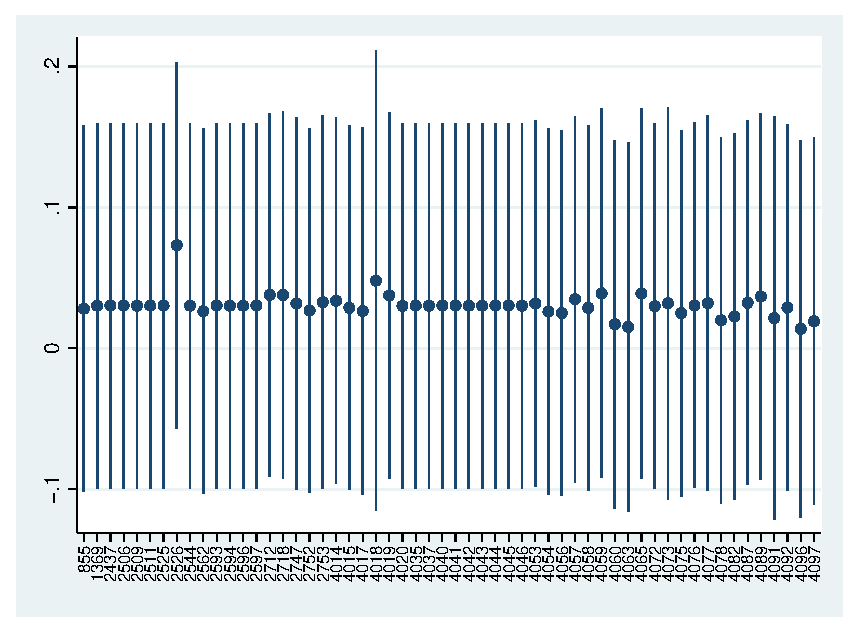
\includegraphics[width=\textwidth]{../../../output/image/coef-interviewer-child-BMI_obese_PmDiD.eps}       
 \caption{Outcome: Not Obese}        
        \end{subfigure}
      \caption{Child Cohort: Droping Each Interviewer}  \label{fig:child-sensitivity-interviewer_PmDiD}
    \end{figure}

    \begin{figure}[H]
      \centering
        \begin{subfigure}[t]{0.75\textwidth}
          \includegraphics[width=\textwidth]{../../../output/image/coef-interviewer-adol-pos_childSDQ_score_PmDiD.eps}       
\caption{Outcome: Positive SDQ Score}        
        \end{subfigure}
        \begin{subfigure}[t]{0.75\textwidth}
          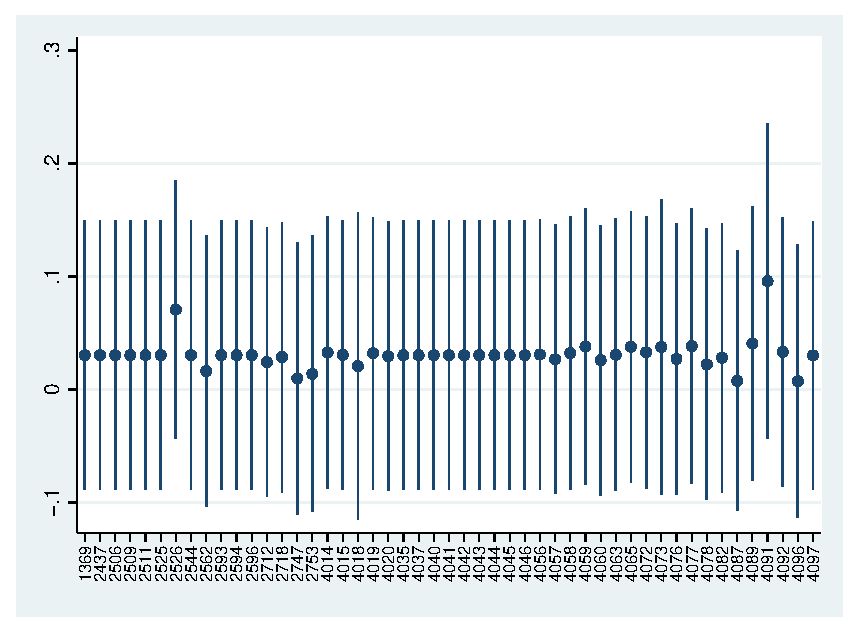
\includegraphics[width=\textwidth]{../../../output/image/coef-interviewer-adol-BMI_obese_PmDiD.eps}       
 \caption{Outcome: Not Obese}        
        \end{subfigure}
      \caption{Adolescent Cohort: Droping Each Interviewer}  \label{fig:adol-sensitivity-interviewer_PmDiD}
    \end{figure}


    \begin{figure}[H]
      \centering
        \begin{subfigure}[t]{0.75\textwidth}
          \includegraphics[width=\textwidth]{../../../output/image/coef-interviewer-adult30-votoMaturita_PmDiD.eps}       
\caption{Outcome: High School Grade}        
        \end{subfigure}
        \begin{subfigure}[t]{0.75\textwidth}
          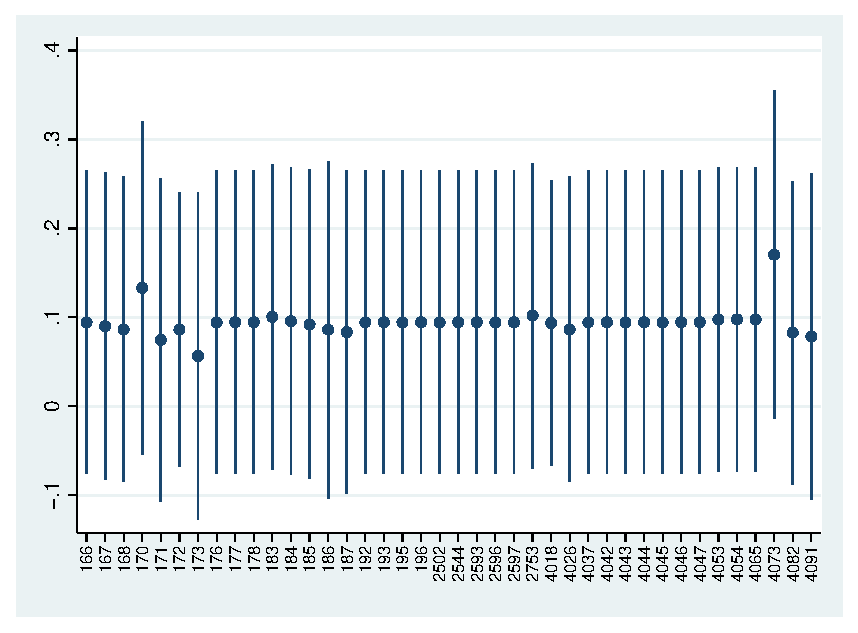
\includegraphics[width=\textwidth]{../../../output/image/coef-interviewer-adult30-BMI_obese_PmDiD.eps}       
 \caption{Outcome: Not Obese}        
        \end{subfigure}
      \caption{Adult-30 Cohort: Droping Each Interviewer}  \label{fig:adult30-sensitivity-interviewer_PmDiD}
    \end{figure}


    \begin{figure}[H]
      \centering
        \begin{subfigure}[t]{0.75\textwidth}
          \includegraphics[width=\textwidth]{../../../output/image/coef-interviewer-adult40-votoMaturita_PmDiD.eps}       
\caption{Outcome: High School Grade}        
        \end{subfigure}
        \begin{subfigure}[t]{0.75\textwidth}
          \includegraphics[width=\textwidth]{../../../output/image/coef-interviewer-adult40-BMI_obese_PmDiD.eps}       
 \caption{Outcome: Not Obese}        
        \end{subfigure}
      \caption{Adult-40 Cohort: Droping Each Interviewer}  \label{fig:adult40-sensitivity-interviewer_PmDiD}
    \end{figure}



\subsubsection{More Detailed Analysis}

\ref{sec:ParmaDiD-analysis} shows some interviewers that show different trend than other interviewers. For child cohort, interviewers 2526 and 4018 show different results for outcomes examined. For adolescent cohort, interviewers 2526, 4018, 4073, and 4091 show some different trends than other interviewers. For adult-30 and adult-40 cohorts, interviewers 187, 4018, and 4073 show some different trends than other interviewers.  In order to examine this more closely, we estimate treatment effects excluding those interviewers on all main outcomes presented in the paper. 




\begin{table}[H] \caption{Estimation Results for Main Outcomes, Child Cohort, DiD with Parma} \label{didpm-M-child-sensitivity}
\scalebox{0.7}{\begin{tabular}{l c c c c}
\toprule
 & None & Drop2526 & Drop4018 & DropAll \\
\midrule
IQ Factor & -0.06 & 0.01 & -0.14 & -0.07 \\
& (0.14) & (0.14) & (0.17) & (0.17) \\
& \textit{ 591 } & \textit{ 549 } & \textit{ 439 } & \textit{ 397 } \\
SDQ Composite - Child & 1.09 & 0.77 & \textbf{ 1.52 } & 1.16 \\
& (0.76) & (0.79) & (0.88) & (0.91) \\
& \textit{ 589 } & \textit{ 547 } & \textit{ 437 } & \textit{ 395 } \\
Not Obese & -0.01 & 0.06 & 0.02 & 0.10 \\
& (0.07) & (0.07) & (0.08) & (0.08) \\
& \textit{ 591 } & \textit{ 549 } & \textit{ 439 } & \textit{ 397 } \\
Not Overweight & -0.02 & -0.02 & -0.01 & -0.02 \\
& (0.06) & (0.06) & (0.07) & (0.08) \\
& \textit{ 591 } & \textit{ 549 } & \textit{ 439 } & \textit{ 397 } \\
Health is Good & 0.07 & 0.05 & 0.05 & 0.02 \\
& (0.08) & (0.08) & (0.09) & (0.10) \\
& \textit{ 590 } & \textit{ 548 } & \textit{ 438 } & \textit{ 396 } \\
Not Excited to Learn & -0.02 & -0.02 & -0.00 & 0.00 \\
& (0.03) & (0.03) & (0.03) & (0.04) \\
& \textit{ 591 } & \textit{ 549 } & \textit{ 439 } & \textit{ 397 } \\
Problems Sitting Still & -0.07 & -0.06 & -0.05 & -0.03 \\
& (0.06) & (0.06) & (0.07) & (0.07) \\
& \textit{ 591 } & \textit{ 549 } & \textit{ 439 } & \textit{ 397 } \\
How Much Child Likes School & \textbf{ 0.20 } & \textbf{ 0.18 } & \textbf{ 0.20 } & \textbf{ 0.18 } \\
& (0.09) & (0.10) & (0.11) & (0.11) \\
& \textit{ 587 } & \textit{ 545 } & \textit{ 435 } & \textit{ 393 } \\
Num. of Friends & -0.22 & -0.17 & 0.06 & 0.11 \\
& (0.49) & (0.51) & (0.66) & (0.70) \\
& \textit{ 578 } & \textit{ 537 } & \textit{ 429 } & \textit{ 388 } \\
Candy Game: Willing to Share Candies & 0.01 & -0.00 & 0.05 & 0.05 \\
& (0.05) & (0.05) & (0.04) & (0.05) \\
& \textit{ 591 } & \textit{ 549 } & \textit{ 439 } & \textit{ 397 } \\
\bottomrule
\end{tabular}
}
\vspace{1ex} \\
\footnotesize\raggedright{\underline{Note 1:} This table shows the estimates of the coefficient for attending Reggio Approach preschools, checking for sensitivity regarding questionable interviewers. Column names indicate the interviewers being dropped. ``DropAll" columns drop all interviewers identified as questionable interviewers in the previous columns.}

\footnotesize\raggedright{\underline{Note 2:} Both unadjusted p-value and stepdown p-value are reported. Bold indicates that the estimate is significant at 10\% level.}
\end{table}




\begin{table}[H] \caption{Estimation Results for Main Outcomes, Adolescent Cohort, DiD with Parma} \label{didpm-M-adol-sensitivity}
\scalebox{0.7}{\begin{tabular}{l c c c c c c}
\toprule
 & None & Drop2526 & Drop4018 & Drop4073 & Drop4091 & DropAll \\
\midrule
IQ Factor & -0.12 & 0.02 & -0.16 & -0.10 & -0.02 & 0.15 \\
& (0.13) & (0.12) & (0.16) & (0.14) & (0.16) & (0.26) \\
& \textit{ 536 } & \textit{ 519 } & \textit{ 417 } & \textit{ 493 } & \textit{ 462 } & \textit{ 283 } \\
SDQ Composite - Child & -0.41 & -0.43 & -0.14 & -1.21 & 0.15 & -0.69 \\
& (0.86) & (0.87) & (1.05) & (0.92) & (0.92) & (1.49) \\
& \textit{ 536 } & \textit{ 519 } & \textit{ 417 } & \textit{ 493 } & \textit{ 462 } & \textit{ 283 } \\
SDQ Composite & 1.04 & 0.92 & \textbf{ 1.61 } & -0.01 & 1.11 & 0.28 \\
& (0.89) & (0.91) & (1.03) & (0.92) & (0.94) & (1.27) \\
& \textit{ 532 } & \textit{ 515 } & \textit{ 413 } & \textit{ 489 } & \textit{ 458 } & \textit{ 279 } \\
Depression Score - positive & \textbf{ 2.26 } & \textbf{ 2.01 } & \textbf{ 2.49 } & \textbf{ 1.69 } & \textbf{ 2.48 } & 1.57 \\
& (1.02) & (1.03) & (1.17) & (1.07) & (1.12) & (1.74) \\
& \textit{ 518 } & \textit{ 501 } & \textit{ 399 } & \textit{ 475 } & \textit{ 445 } & \textit{ 266 } \\
Locus of Control - positive & \textbf{ -0.23 } & \textbf{ -0.26 } & \textbf{ -0.25 } & -0.04 & -0.22 & 0.21 \\
& (0.14) & (0.14) & (0.15) & (0.14) & (0.16) & (0.20) \\
& \textit{ 528 } & \textit{ 511 } & \textit{ 409 } & \textit{ 485 } & \textit{ 454 } & \textit{ 275 } \\
Not Obese & 0.03 & 0.06 & 0.03 & 0.03 & \textbf{ 0.11 } & \textbf{ 0.23 } \\
& (0.06) & (0.06) & (0.07) & (0.07) & (0.07) & (0.11) \\
& \textit{ 536 } & \textit{ 519 } & \textit{ 417 } & \textit{ 493 } & \textit{ 462 } & \textit{ 283 } \\
Not Overweight & \textbf{ 0.08 } & \textbf{ 0.08 } & \textbf{ 0.10 } & \textbf{ 0.07 } & 0.06 & 0.05 \\
& (0.04) & (0.04) & (0.05) & (0.04) & (0.04) & (0.06) \\
& \textit{ 536 } & \textit{ 519 } & \textit{ 417 } & \textit{ 493 } & \textit{ 462 } & \textit{ 283 } \\
Health is Good & 0.10 & 0.10 & 0.08 & \textbf{ 0.21 } & 0.12 & \textbf{ 0.32 } \\
& (0.09) & (0.09) & (0.10) & (0.09) & (0.10) & (0.14) \\
& \textit{ 535 } & \textit{ 518 } & \textit{ 416 } & \textit{ 492 } & \textit{ 461 } & \textit{ 282 } \\
Go To School & 0.03 & 0.02 & 0.02 & 0.03 & \textbf{ 0.06 } & 0.02 \\
& (0.03) & (0.03) & (0.04) & (0.04) & (0.04) & (0.05) \\
& \textit{ 536 } & \textit{ 519 } & \textit{ 417 } & \textit{ 493 } & \textit{ 462 } & \textit{ 283 } \\
How Much Child Likes School & -0.08 & -0.12 & 0.06 & \textbf{ -0.27 } & -0.03 & -0.05 \\
& (0.16) & (0.16) & (0.18) & (0.17) & (0.18) & (0.23) \\
& \textit{ 514 } & \textit{ 499 } & \textit{ 397 } & \textit{ 471 } & \textit{ 444 } & \textit{ 269 } \\
Days of Sport (Weekly) & \textbf{ -0.66 } & \textbf{ -0.52 } & \textbf{ -0.84 } & \textbf{ -0.56 } & \textbf{ -0.55 } & -0.52 \\
& (0.32) & (0.32) & (0.36) & (0.34) & (0.34) & (0.48) \\
& \textit{ 522 } & \textit{ 506 } & \textit{ 406 } & \textit{ 479 } & \textit{ 448 } & \textit{ 273 } \\
Num. of Friends & -2.52 & -2.23 & -1.77 & -1.09 & -0.59 & 4.59 \\
& (1.85) & (1.87) & (2.06) & (2.00) & (1.85) & (3.28) \\
& \textit{ 512 } & \textit{ 495 } & \textit{ 396 } & \textit{ 469 } & \textit{ 441 } & \textit{ 265 } \\
Volunteers & -0.04 & -0.02 & -0.03 & -0.02 & -0.04 & 0.04 \\
& (0.08) & (0.08) & (0.09) & (0.09) & (0.09) & (0.13) \\
& \textit{ 536 } & \textit{ 519 } & \textit{ 417 } & \textit{ 493 } & \textit{ 462 } & \textit{ 283 } \\
Trust Score & 0.30 & \textbf{ 0.40 } & 0.35 & -0.04 & 0.30 & 0.00 \\
& (0.26) & (0.26) & (0.30) & (0.26) & (0.30) & (0.39) \\
& \textit{ 532 } & \textit{ 515 } & \textit{ 413 } & \textit{ 489 } & \textit{ 458 } & \textit{ 279 } \\
\bottomrule
\end{tabular}
}
\vspace{1ex} \\
\footnotesize\raggedright{\underline{Note 1:} This table shows the estimates of the coefficient for attending Reggio Approach preschools, checking for sensitivity regarding questionable interviewers. Column names indicate the interviewers being dropped. ``DropAll" columns drop all interviewers identified as questionable interviewers in the previous columns.}

\footnotesize\raggedright{\underline{Note 2:} Both unadjusted p-value and stepdown p-value are reported. Bold indicates that the estimate is significant at 10\% level.}
\end{table}




\begin{table}[H] \caption{Estimation Results for Main Outcomes, Adult-30 Cohort, DiD with Parma} \label{didpm-M-adult30-sensitivity}
\scalebox{0.7}{\begin{tabular}{l c c c c c}
\toprule
 & None & Drop187 & Drop4018 & Drop4073 & DropAll \\
\midrule
IQ Factor & \textbf{ -0.30 } & -0.23 & \textbf{ -0.35 } & \textbf{ -0.28 } & -0.24 \\
& (0.18) & (0.20) & (0.19) & (0.18) & (0.20) \\
& \textit{ 300 } & \textit{ 269 } & \textit{ 294 } & \textit{ 286 } & \textit{ 249 } \\
Graduate from High School & 0.04 & 0.05 & 0.06 & 0.06 & 0.10 \\
& (0.08) & (0.08) & (0.08) & (0.08) & (0.09) \\
& \textit{ 300 } & \textit{ 269 } & \textit{ 294 } & \textit{ 286 } & \textit{ 249 } \\
High School Grade & 1.89 & -0.34 & 3.68 & 3.21 & 3.79 \\
& (3.50) & (3.69) & (3.49) & (2.67) & (2.70) \\
& \textit{ 248 } & \textit{ 217 } & \textit{ 242 } & \textit{ 234 } & \textit{ 197 } \\
High School Grade (Standardized) & 3.81 & 2.64 & \textbf{ 5.04 } & \textbf{ 3.70 } & \textbf{ 4.17 } \\
& (2.78) & (2.99) & (2.82) & (2.38) & (2.62) \\
& \textit{ 243 } & \textit{ 212 } & \textit{ 237 } & \textit{ 232 } & \textit{ 195 } \\
Max Edu: University & 0.07 & 0.07 & 0.11 & 0.09 & 0.14 \\
& (0.11) & (0.11) & (0.11) & (0.11) & (0.11) \\
& \textit{ 300 } & \textit{ 269 } & \textit{ 294 } & \textit{ 286 } & \textit{ 249 } \\
Employed & 0.11 & 0.09 & \textbf{ 0.13 } & 0.09 & 0.11 \\
& (0.08) & (0.08) & (0.08) & (0.08) & (0.08) \\
& \textit{ 300 } & \textit{ 269 } & \textit{ 294 } & \textit{ 286 } & \textit{ 249 } \\
Hours Worked Per Week & 3.20 & 2.60 & 4.11 & 2.23 & 2.73 \\
& (3.63) & (3.85) & (3.65) & (3.78) & (4.02) \\
& \textit{ 267 } & \textit{ 236 } & \textit{ 264 } & \textit{ 253 } & \textit{ 219 } \\
Married or Cohabitating & 0.16 & \textbf{ 0.20 } & 0.14 & \textbf{ 0.19 } & \textbf{ 0.21 } \\
& (0.11) & (0.12) & (0.12) & (0.12) & (0.13) \\
& \textit{ 300 } & \textit{ 269 } & \textit{ 294 } & \textit{ 286 } & \textit{ 249 } \\
Not Obese & 0.01 & 0.01 & -0.01 & 0.01 & -0.01 \\
& (0.10) & (0.10) & (0.09) & (0.10) & (0.10) \\
& \textit{ 300 } & \textit{ 269 } & \textit{ 294 } & \textit{ 286 } & \textit{ 249 } \\
Not Overweight & 0.07 & 0.02 & 0.09 & 0.05 & 0.03 \\
& (0.10) & (0.10) & (0.10) & (0.10) & (0.11) \\
& \textit{ 300 } & \textit{ 269 } & \textit{ 294 } & \textit{ 286 } & \textit{ 249 } \\
Locus of Control - positive & \textbf{ 0.34 } & 0.29 & \textbf{ 0.32 } & \textbf{ 0.37 } & 0.30 \\
& (0.22) & (0.23) & (0.22) & (0.24) & (0.25) \\
& \textit{ 286 } & \textit{ 255 } & \textit{ 280 } & \textit{ 272 } & \textit{ 235 } \\
Depression Score - positive & 0.89 & 0.74 & 1.24 & 1.10 & 1.28 \\
& (1.34) & (1.38) & (1.40) & (1.30) & (1.38) \\
& \textit{ 298 } & \textit{ 267 } & \textit{ 292 } & \textit{ 284 } & \textit{ 247 } \\
Volunteers & -0.04 & -0.01 & -0.04 & -0.06 & -0.03 \\
& (0.09) & (0.10) & (0.10) & (0.10) & (0.11) \\
& \textit{ 300 } & \textit{ 269 } & \textit{ 294 } & \textit{ 286 } & \textit{ 249 } \\
Ever Voted for Municipal & -0.06 & -0.02 & 0.00 & -0.07 & 0.05 \\
& (0.09) & (0.09) & (0.09) & (0.09) & (0.10) \\
& \textit{ 296 } & \textit{ 265 } & \textit{ 290 } & \textit{ 282 } & \textit{ 245 } \\
Ever Voted for Regional & -0.06 & -0.06 & -0.03 & -0.07 & -0.01 \\
& (0.09) & (0.09) & (0.09) & (0.09) & (0.10) \\
& \textit{ 296 } & \textit{ 265 } & \textit{ 290 } & \textit{ 282 } & \textit{ 245 } \\
Num. of Friends & \textbf{ 3.21 } & \textbf{ 3.06 } & \textbf{ 2.65 } & \textbf{ 3.53 } & \textbf{ 3.00 } \\
& (1.67) & (1.83) & (1.68) & (1.69) & (1.87) \\
& \textit{ 281 } & \textit{ 251 } & \textit{ 275 } & \textit{ 267 } & \textit{ 231 } \\
Trust Score & \textbf{ 0.59 } & \textbf{ 0.86 } & \textbf{ 0.62 } & \textbf{ 0.73 } & \textbf{ 1.04 } \\
& (0.40) & (0.41) & (0.42) & (0.38) & (0.41) \\
& \textit{ 298 } & \textit{ 267 } & \textit{ 292 } & \textit{ 284 } & \textit{ 247 } \\
\bottomrule
\end{tabular}
}
\vspace{1ex} \\
\footnotesize\raggedright{\underline{Note 1:} This table shows the estimates of the coefficient for attending Reggio Approach preschools, checking for sensitivity regarding questionable interviewers. Column names indicate the interviewers being dropped. ``DropAll" columns drop all interviewers identified as questionable interviewers in the previous columns.}

\footnotesize\raggedright{\underline{Note 2:} Both unadjusted p-value and stepdown p-value are reported. Bold indicates that the estimate is significant at 10\% level.}
\end{table}


\begin{table}[H] \caption{Estimation Results for Main Outcomes, Adult-40 Cohort, DiD with Parma} \label{didpm-M-adult40-sensitivity}
\scalebox{0.7}{\begin{tabular}{l c c c c c}
\toprule
 & None & Drop187 & Drop4018 & Drop4073 & DropAll \\
\midrule
IQ Factor & \textbf{ -0.31 } & \textbf{ -0.39 } & \textbf{ -0.28 } & \textbf{ -0.29 } & \textbf{ -0.35 } \\
& (0.16) & (0.17) & (0.19) & (0.14) & (0.16) \\
& \textit{ 273 } & \textit{ 251 } & \textit{ 246 } & \textit{ 258 } & \textit{ 209 } \\
Graduate from High School & 0.05 & 0.00 & 0.08 & 0.11 & 0.11 \\
& (0.09) & (0.09) & (0.11) & (0.09) & (0.12) \\
& \textit{ 273 } & \textit{ 251 } & \textit{ 246 } & \textit{ 258 } & \textit{ 209 } \\
High School Grade & 1.66 & -1.91 & \textbf{ 7.00 } & 2.10 & 3.15 \\
& (3.25) & (3.45) & (3.59) & (2.90) & (3.33) \\
& \textit{ 215 } & \textit{ 193 } & \textit{ 190 } & \textit{ 205 } & \textit{ 158 } \\
High School Grade (Standardized) & 1.46 & -1.59 & \textbf{ 5.00 } & 1.39 & 1.45 \\
& (2.74) & (2.87) & (3.02) & (2.53) & (2.96) \\
& \textit{ 212 } & \textit{ 191 } & \textit{ 188 } & \textit{ 203 } & \textit{ 158 } \\
Max Edu: University & -0.06 & -0.07 & 0.01 & -0.03 & 0.04 \\
& (0.11) & (0.11) & (0.12) & (0.11) & (0.13) \\
& \textit{ 273 } & \textit{ 251 } & \textit{ 246 } & \textit{ 258 } & \textit{ 209 } \\
Employed & 0.01 & 0.00 & -0.02 & 0.03 & -0.02 \\
& (0.05) & (0.05) & (0.04) & (0.05) & (0.05) \\
& \textit{ 273 } & \textit{ 251 } & \textit{ 246 } & \textit{ 258 } & \textit{ 209 } \\
Hours Worked Per Week & -1.70 & -1.40 & -2.41 & -1.21 & -1.72 \\
& (2.53) & (2.72) & (2.46) & (2.68) & (2.95) \\
& \textit{ 252 } & \textit{ 231 } & \textit{ 230 } & \textit{ 237 } & \textit{ 194 } \\
Married or Cohabitating & -0.09 & -0.07 & -0.08 & -0.09 & -0.03 \\
& (0.12) & (0.12) & (0.13) & (0.12) & (0.15) \\
& \textit{ 273 } & \textit{ 251 } & \textit{ 246 } & \textit{ 258 } & \textit{ 209 } \\
Not Obese & 0.14 & 0.09 & 0.00 & 0.15 & -0.00 \\
& (0.11) & (0.12) & (0.10) & (0.12) & (0.12) \\
& \textit{ 273 } & \textit{ 251 } & \textit{ 246 } & \textit{ 258 } & \textit{ 209 } \\
Not Overweight & -0.09 & -0.05 & -0.02 & -0.07 & 0.06 \\
& (0.11) & (0.12) & (0.14) & (0.12) & (0.16) \\
& \textit{ 273 } & \textit{ 251 } & \textit{ 246 } & \textit{ 258 } & \textit{ 209 } \\
Locus of Control - positive & -0.01 & -0.03 & 0.27 & -0.07 & 0.19 \\
& (0.22) & (0.24) & (0.26) & (0.22) & (0.30) \\
& \textit{ 267 } & \textit{ 245 } & \textit{ 240 } & \textit{ 252 } & \textit{ 203 } \\
Depression Score - positive & 2.06 & 1.33 & \textbf{ 3.45 } & 2.20 & \textbf{ 2.97 } \\
& (1.45) & (1.51) & (1.72) & (1.54) & (1.98) \\
& \textit{ 270 } & \textit{ 248 } & \textit{ 243 } & \textit{ 255 } & \textit{ 206 } \\
Volunteers & 0.06 & 0.11 & 0.12 & 0.07 & \textbf{ 0.19 } \\
& (0.09) & (0.10) & (0.09) & (0.10) & (0.11) \\
& \textit{ 273 } & \textit{ 251 } & \textit{ 246 } & \textit{ 258 } & \textit{ 209 } \\
Ever Voted for Municipal & 0.05 & -0.00 & \textbf{ 0.25 } & 0.05 & 0.15 \\
& (0.11) & (0.11) & (0.11) & (0.12) & (0.11) \\
& \textit{ 265 } & \textit{ 243 } & \textit{ 238 } & \textit{ 250 } & \textit{ 201 } \\
Ever Voted for Regional & 0.11 & 0.01 & \textbf{ 0.25 } & 0.11 & 0.13 \\
& (0.11) & (0.11) & (0.11) & (0.12) & (0.12) \\
& \textit{ 265 } & \textit{ 243 } & \textit{ 238 } & \textit{ 250 } & \textit{ 201 } \\
Num. of Friends & \textbf{ 2.43 } & 1.12 & \textbf{ 2.16 } & \textbf{ 2.91 } & 1.19 \\
& (1.33) & (1.32) & (1.47) & (1.42) & (1.65) \\
& \textit{ 248 } & \textit{ 226 } & \textit{ 221 } & \textit{ 233 } & \textit{ 184 } \\
Trust Score & 0.28 & 0.43 & 0.24 & 0.22 & 0.52 \\
& (0.40) & (0.43) & (0.47) & (0.39) & (0.51) \\
& \textit{ 273 } & \textit{ 251 } & \textit{ 246 } & \textit{ 258 } & \textit{ 209 } \\
\bottomrule
\end{tabular}
}
\vspace{1ex} \\
\footnotesize\raggedright{\underline{Note 1:} This table shows the estimates of the coefficient for attending Reggio Approach preschools, checking for sensitivity regarding questionable interviewers. Column names indicate the interviewers being dropped. ``DropAll" columns drop all interviewers identified as questionable interviewers in the previous columns.}

\footnotesize\raggedright{\underline{Note 2:} Both unadjusted p-value and stepdown p-value are reported. Bold indicates that the estimate is significant at 10\% level.}
\end{table}



\end{document}
